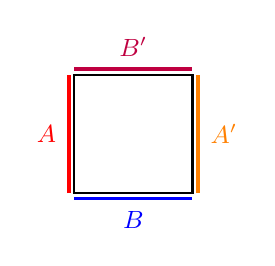
\begin{tikzpicture}[line width=0.8pt, every node/.style={font=\small}]
  \draw (0,0) rectangle (1.5,1.5);
  \draw[red, line width=1.4pt] (-0.07,0) -- (-0.07,1.5);
  \node[red, left] at (-0.1,0.75) {$A$};
  \draw[orange, line width=1.4pt] (1.57,0) -- (1.57,1.5);
  \node[orange, right] at (1.6,0.75) {$A'$};
  \draw[blue, line width=1.4pt] (0,-0.07) -- (1.5,-0.07);
  \node[blue, below] at (0.75,-0.1) {$B$};
  \draw[purple, line width=1.4pt] (0,1.57) -- (1.5,1.57);
  \node[purple, above] at (0.75,1.6) {$B'$};
\end{tikzpicture}
